\chapter{Atom dan Molekul}\label{ch:g7:atoms-and-molecules}

Ambillah setetes air dan potonglah menjadi dua. Setiap belahannya masih
air. Potong lagi sebelahnya menjadi dua, lagi, dan lagi. Dapatkah kamu
terus melakukannya selamanya, atau akankah kamu sampai pada sepotong
yang begitu kecil sehingga memotongnya sekali lagi menghasilkan sesuatu
yang sama sekali bukan air? Sekitar tahun 400~SM, pemikir Yunani
Demokritos menebak jawabannya: materi tersusun atas kepingan-kepingan
sangat kecil yang tidak dapat dipotong, yang disebutnya \emph{\omterm{def:g7:atoms-and-molecules:atom}{atom}},
dari kata Yunani untuk ``tak terpotong''. Diperlukan lebih dari dua ribu
tahun, dan kerja para ahli kimia abad kesembilan belas, untuk mengubah
tebakan itu menjadi ilmu. Bab ini menguraikan kepingan-kepingan itu ---
\omterm{def:g7:atoms-and-molecules:atom}{atom} --- dan cara \omterm{def:g7:atoms-and-molecules:atom}{atom-atom} berkelompok menjadi \omterm{def:g7:atoms-and-molecules:molecule}{molekul}.

\begin{recall}
\omterm{def:g6:pure-substances-and-mixtures:pure-substance}{Zat murni}, seperti air atau oksigen, tersusun atas satu \omterm{def:g6:pure-substances-and-mixtures:species}{spesies kimia}
saja; \omterm{def:g6:pure-substances-and-mixtures:mixture}{campuran}, seperti \omterm{def:g4:air-a-mixture-of-gases:air}{udara}, mengandung beberapa spesies
(\cref{ch:g6:pure-substances-and-mixtures}). \omterm{def:g4:air-a-mixture-of-gases:air}{Udara} terdiri atas
sekitar empat perlima nitrogen dan seperlima oksigen
(\cref{ch:g4:air-a-mixture-of-gases}).
\end{recall}

\section{Atom}

\begin{definition}[Atom]\label{def:g7:atoms-and-molecules:atom}
Semua materi tersusun atas partikel-partikel yang sangat kecil yang
disebut \emph{atom}\index{atom}. Di alam hanya ada sekitar seratus
jenis atom yang berbeda, dan setiap zat --- air, \omterm{def:g4:air-a-mixture-of-gases:air}{udara}, besi, gula,
tubuh kita sendiri --- tersusun atas atom-atom dari beberapa jenis itu.
\end{definition}

\begin{proposition}[Atom itu sangat kecil]\label{prop:g7:atoms-and-molecules:tiny}
% ledger: const:a0, earth:diameter (8 cm apple: 12756 km / 8 cm = 1.6 x 10^8;
% 0.1-0.15 nm x 1.6 x 10^8 = 1.7-2.4 cm, a small cherry)
\omterm{def:g7:atoms-and-molecules:atom}{Atom} terkecil, \omterm{def:g7:atoms-and-molecules:atom}{atom} hidrogen, berukuran sekitar sepersepuluh juta
milimeter; \omterm{def:g7:atoms-and-molecules:atom}{atom-atom} lainnya paling besar hanya beberapa kali lebih
besar. Sepuluh juta \omterm{def:g7:atoms-and-molecules:atom}{atom} hidrogen yang dijajarkan akan membentuk garis
sepanjang satu milimeter. Untuk membayangkannya: seandainya sebutir
apel diperbesar sampai seukuran Bumi, setiap \omterm{def:g7:atoms-and-molecules:atom}{atomnya} akan kira-kira
sebesar buah ceri kecil.
\end{proposition}

\begin{remark}[Terlihat tanpa dilihat]\label{rem:g7:atoms-and-molecules:seen}
Tidak ada mikroskop cahaya yang dapat memperlihatkan \omterm{def:g7:atoms-and-molecules:atom}{atom}: \omterm{def:g7:atoms-and-molecules:atom}{atom} jauh
lebih kecil daripada gelombang cahaya. Sejak tahun 1980-an, mikroskop
khusus yang meraba permukaan dengan ujung jarum yang sangat halus telah
menghasilkan gambar tempat \omterm{def:g7:atoms-and-molecules:atom}{atom-atom} tunggal tampak sebagai tonjolan.
\end{remark}

\begin{definition}[Lambang atom]\label{def:g7:atoms-and-molecules:symbol}
Setiap jenis \omterm{def:g7:atoms-and-molecules:atom}{atom} memiliki nama dan \emph{lambang}\index{lambang atom}:
satu huruf kapital, kadang diikuti satu huruf kecil. Lambang itu sama
dalam semua bahasa.
\end{definition}

\begin{center}
\small
\begin{tabular}{llll|llll}
\hline
\omterm{def:g7:atoms-and-molecules:atom}{atom} & \omterm{def:g7:atoms-and-molecules:symbol}{lambang} & & warna model & \omterm{def:g7:atoms-and-molecules:atom}{atom} & \omterm{def:g7:atoms-and-molecules:symbol}{lambang} & & warna model \\
\hline
hidrogen & \ce{H} & \tikz\node[aH]{}; & putih & natrium & \ce{Na} & \tikz\node[aNa]{}; & ungu \\
karbon & \ce{C} & \tikz\node[aC]{}; & hitam & belerang & \ce{S} & \tikz\node[aS]{}; & kuning \\
nitrogen & \ce{N} & \tikz\node[aN]{}; & biru & klorin & \ce{Cl} & \tikz\node[aCl]{}; & hijau \\
oksigen & \ce{O} & \tikz\node[aO]{}; & merah & besi, tembaga & \ce{Fe}, \ce{Cu} & & --- \\
\hline
\end{tabular}
\end{center}

\begin{remark}[Asal-usul lambang]\label{rem:g7:atoms-and-molecules:latin}
Kebanyakan \omterm{def:g7:atoms-and-molecules:symbol}{lambang} adalah huruf pertama nama \omterm{def:g7:atoms-and-molecules:atom}{atomnya}: \ce{H} untuk
hidrogen, \ce{C} untuk karbon, \ce{O} untuk oksigen. Sebagian berasal
dari nama Latin yang lebih tua: \ce{Na} untuk natrium (\emph{natrium},
nama yang juga dipakai dalam bahasa Indonesia), \ce{Fe} untuk besi
(\emph{ferrum}), \ce{Cu} untuk tembaga (\emph{cuprum}). Huruf kedua
selalu huruf kecil: \ce{Co} adalah \omterm{def:g7:atoms-and-molecules:atom}{atom} kobalt, sedangkan CO, dengan O
kapital, adalah sesuatu yang sama sekali lain.
\end{remark}

\begin{history}[Atom-atom Dalton, 1808]
Pada tahun 1808 ahli kimia John Dalton menerbitkan tabel \omterm{def:g7:atoms-and-molecules:atom}{atom-atom} yang
dikenal pada masa itu, masing-masing digambar sebagai lingkaran kecil
dengan tandanya sendiri. Dialah yang pertama mengatakan bahwa setiap
\omterm{def:g7:atoms-and-molecules:atom}{atom} dari satu jenis memiliki berat yang sama, dan bahwa para ahli kimia
dapat membandingkan berat-berat itu. Tetapi ia juga menduga bahwa air
adalah satu \omterm{def:g7:atoms-and-molecules:atom}{atom} hidrogen yang tergabung dengan satu \omterm{def:g7:atoms-and-molecules:atom}{atom} oksigen;
diperlukan lima puluh tahun lagi sampai para ahli kimia sepakat bahwa
sebuah \omterm{def:g7:atoms-and-molecules:molecule}{molekul} air mengandung \emph{dua} \omterm{def:g7:atoms-and-molecules:atom}{atom} hidrogen.
\end{history}

\begin{omfigure}
\begin{minipage}[b]{0.3\linewidth}\centering
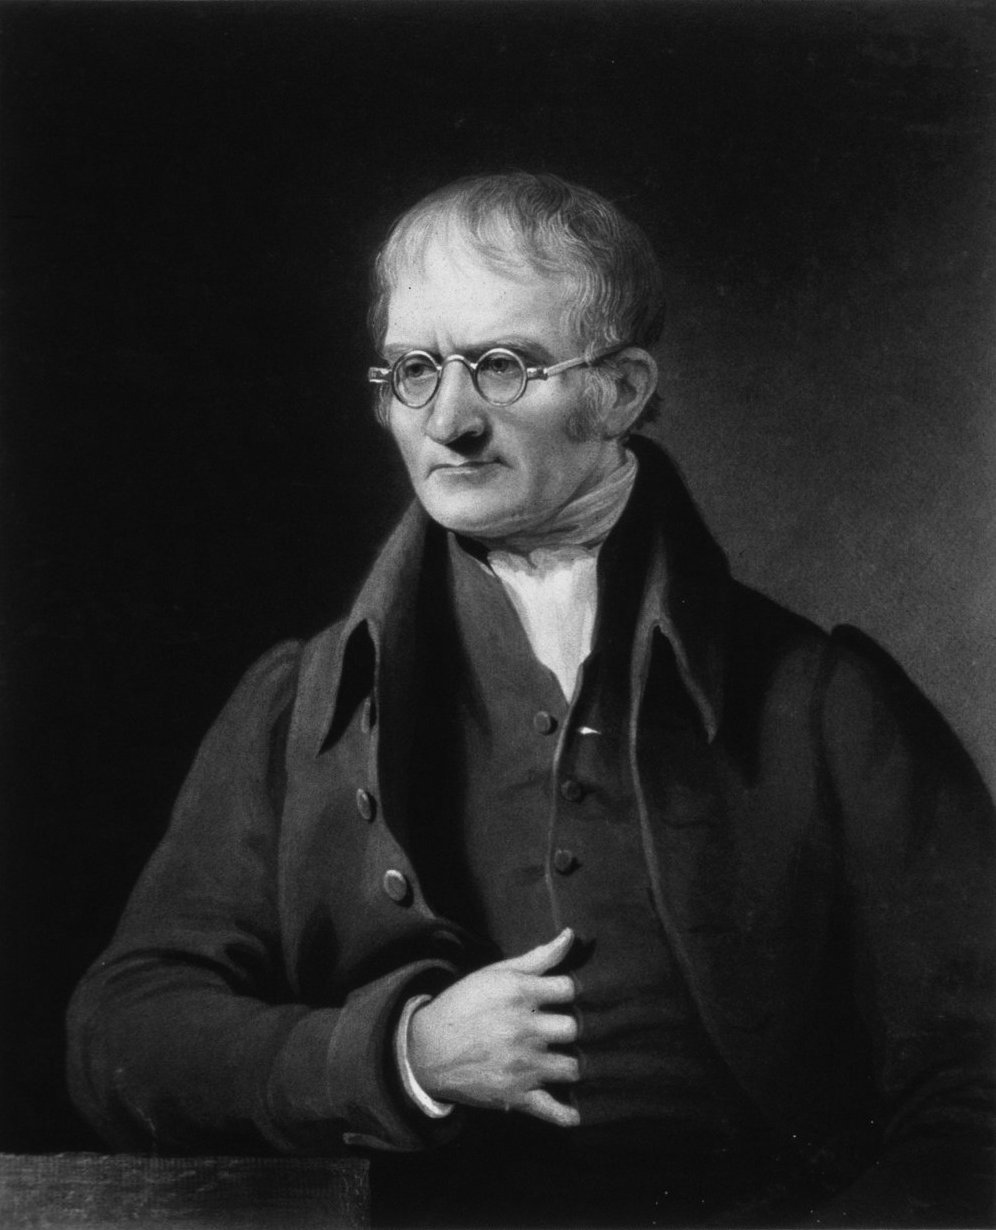
\includegraphics[width=\linewidth]{images/book1/dalton.jpg}

{\small John Dalton (1766--1844).}
\end{minipage}\hfill
\begin{minipage}[b]{0.66\linewidth}\centering
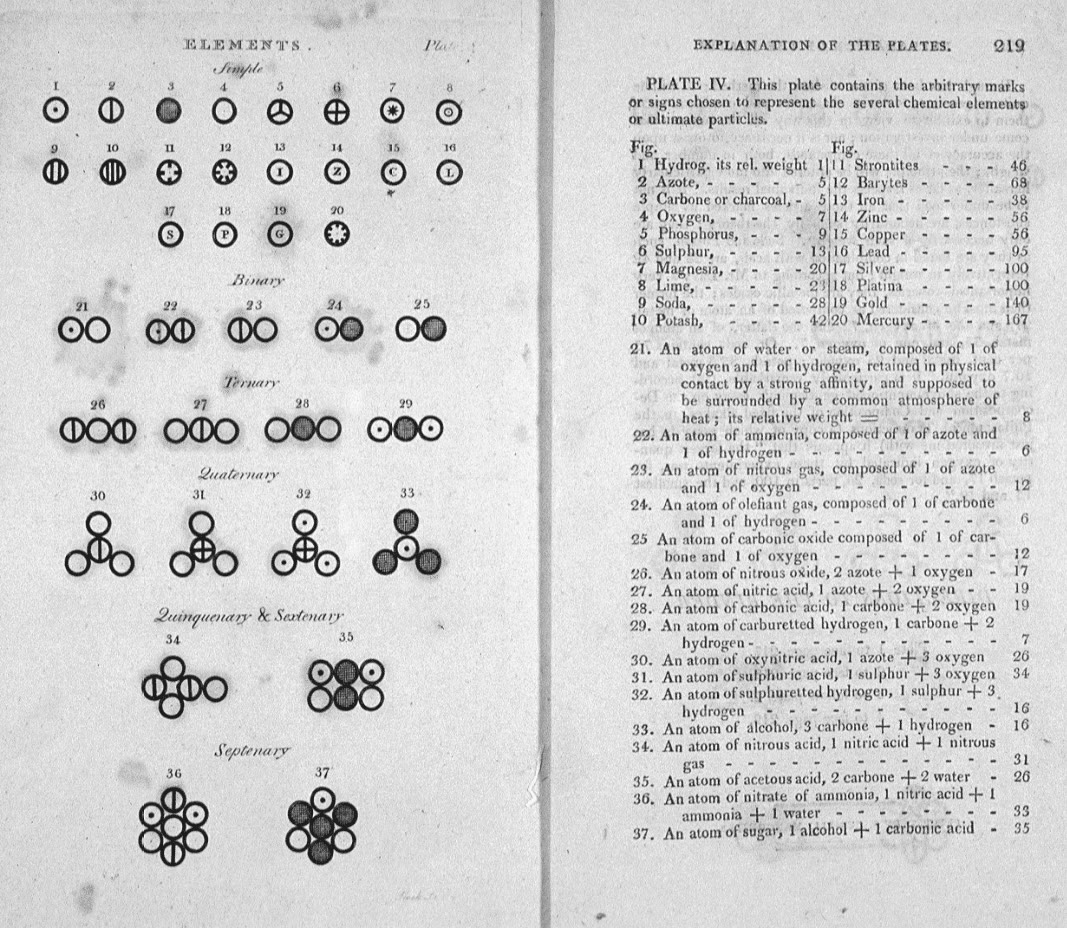
\includegraphics[width=\linewidth]{images/book1/dalton-symbols.jpg}

{\small Tabel Dalton tahun 1808: air menurut Dalton, tanda 21, adalah
satu lingkaran hidrogen di samping satu lingkaran oksigen.}
\end{minipage}
\end{omfigure}

\section{Molekul}

\begin{definition}[Molekul]\label{def:g7:atoms-and-molecules:molecule}
Sebuah \emph{molekul}\index{molekul} adalah sekelompok \omterm{def:g7:atoms-and-molecules:atom}{atom} yang terikat
erat satu sama lain. Molekul adalah bagian terkecil sebuah zat yang
masih merupakan zat itu: sebuah molekul air adalah jumlah air terkecil
yang mungkin.
\end{definition}

\begin{example}[Tujuh molekul]\label{ex:g7:atoms-and-molecules:seven}
\begin{itemize}
  \item \omterm{def:g7:atoms-and-molecules:molecule}{molekul} \emph{hidrogen}: dua \omterm{def:g7:atoms-and-molecules:atom}{atom} hidrogen;
  \item \omterm{def:g7:atoms-and-molecules:molecule}{molekul} \emph{oksigen}, yang kita hirup: dua \omterm{def:g7:atoms-and-molecules:atom}{atom} oksigen;
  \item \omterm{def:g7:atoms-and-molecules:molecule}{molekul} \emph{nitrogen}, empat perlima \omterm{def:g4:air-a-mixture-of-gases:air}{udara}: dua \omterm{def:g7:atoms-and-molecules:atom}{atom}
        nitrogen;
  \item \omterm{def:g7:atoms-and-molecules:molecule}{molekul} \emph{air}: dua \omterm{def:g7:atoms-and-molecules:atom}{atom} hidrogen dan satu \omterm{def:g7:atoms-and-molecules:atom}{atom} oksigen;
  \item \omterm{def:g7:atoms-and-molecules:molecule}{molekul} \emph{karbon dioksida}, yang kita embuskan: satu \omterm{def:g7:atoms-and-molecules:atom}{atom}
        karbon dan dua \omterm{def:g7:atoms-and-molecules:atom}{atom} oksigen;
  \item \omterm{def:g7:atoms-and-molecules:molecule}{molekul} \emph{metana}, bagian utama gas alam yang dibakar di
        kompor gas: satu \omterm{def:g7:atoms-and-molecules:atom}{atom} karbon dan empat \omterm{def:g7:atoms-and-molecules:atom}{atom} hidrogen;
  \item \omterm{def:g7:atoms-and-molecules:molecule}{molekul} \emph{dinitrogen oksida}, gas pembius: dua \omterm{def:g7:atoms-and-molecules:atom}{atom} nitrogen
        dan satu \omterm{def:g7:atoms-and-molecules:atom}{atom} oksigen.
\end{itemize}
\end{example}

\begin{omfigure}
\begin{tikzpicture}[font=\small]
  % hydrogen
  \begin{scope}[xshift=0cm]
    \node[aH] (a) at (-0.25,0) {}; \node[aH] (b) at (0.25,0) {};
    \begin{scope}[on background layer]\draw[bond] (a.center) -- (b.center);\end{scope}
    \node at (0,-1.05) {hidrogen};
  \end{scope}
  % oxygen
  \begin{scope}[xshift=2.6cm]
    \node[aO] (a) at (-0.33,0) {}; \node[aO] (b) at (0.33,0) {};
    \begin{scope}[on background layer]
      \draw[bond, line width=1.1pt] ([yshift=1.6pt]a.center) -- ([yshift=1.6pt]b.center);
      \draw[bond, line width=1.1pt] ([yshift=-1.6pt]a.center) -- ([yshift=-1.6pt]b.center);
    \end{scope}
    \node at (0,-1.05) {oksigen};
  \end{scope}
  % nitrogen
  \begin{scope}[xshift=5.2cm]
    \node[aN] (a) at (-0.33,0) {}; \node[aN] (b) at (0.33,0) {};
    \begin{scope}[on background layer]
      \foreach \d in {-2.4,0,2.4}
        \draw[bond, line width=0.9pt] ([yshift=\d pt]a.center) -- ([yshift=\d pt]b.center);
    \end{scope}
    \node at (0,-1.05) {nitrogen};
  \end{scope}
  % water
  \begin{scope}[xshift=7.8cm, yshift=0.2cm]
    \node[aO] (o) at (0,0) {};
    \node[aH] (h1) at (-0.62,-0.48) {}; \node[aH] (h2) at (0.62,-0.48) {};
    \begin{scope}[on background layer]
      \draw[bond] (o.center) -- (h1.center); \draw[bond] (o.center) -- (h2.center);
    \end{scope}
    \node at (0,-1.25) {air};
  \end{scope}
  % carbon dioxide
  \begin{scope}[xshift=0.9cm, yshift=-2.7cm]
    \node[aO] (a) at (-0.85,0) {}; \node[aC] (c) at (0,0) {}; \node[aO] (b) at (0.85,0) {};
    \begin{scope}[on background layer]
      \foreach \d in {-1.6,1.6} {
        \draw[bond, line width=1.1pt] ([yshift=\d pt]a.center) -- ([yshift=\d pt]c.center);
        \draw[bond, line width=1.1pt] ([yshift=\d pt]c.center) -- ([yshift=\d pt]b.center);}
    \end{scope}
    \node at (0,-1.05) {karbon dioksida};
  \end{scope}
  % methane
  \begin{scope}[xshift=4.4cm, yshift=-2.6cm]
    \node[aC] (c) at (0,0) {};
    \node[aH] (h1) at (0,0.78) {};
    \node[aH] (h2) at (-0.74,-0.3) {};
    \node[aH] (h3) at (0.74,-0.3) {};
    \begin{scope}[on background layer]
      \draw[bond] (c.center) -- (h1.center); \draw[bond] (c.center) -- (h2.center);
      \draw[bond] (c.center) -- (h3.center);
    \end{scope}
    \draw[bond] (c.center) -- (0.22,-0.52);
    \node[aH] at (0.24,-0.58) {};
    \node at (0,-1.15) {metana};
  \end{scope}
  % nitrous oxide
  \begin{scope}[xshift=7.8cm, yshift=-2.7cm]
    \node[aN] (a) at (-0.8,0) {}; \node[aN] (b) at (0,0) {}; \node[aO] (c) at (0.8,0) {};
    \begin{scope}[on background layer]
      \foreach \d in {-1.6,1.6} {
        \draw[bond, line width=1.1pt] ([yshift=\d pt]a.center) -- ([yshift=\d pt]b.center);
        \draw[bond, line width=1.1pt] ([yshift=\d pt]b.center) -- ([yshift=\d pt]c.center);}
    \end{scope}
    \node at (0,-1.05) {dinitrogen oksida};
  \end{scope}
\end{tikzpicture}

{\small Model bola dan tongkat ketujuh \omterm{def:g7:atoms-and-molecules:molecule}{molekul} pada
\cref{ex:g7:atoms-and-molecules:seven}. Setiap tongkat melambangkan
ikatan antara dua \omterm{def:g7:atoms-and-molecules:atom}{atom}; mengapa sebagian \omterm{def:g7:atoms-and-molecules:atom}{atom} berbagi dua atau tiga
tongkat dijelaskan di bab berikutnya.}
\end{omfigure}

\begin{proposition}[Molekul zat murni dan molekul campuran]\label{prop:g7:atoms-and-molecules:pure}
Dalam \omterm{def:g6:pure-substances-and-mixtures:pure-substance}{zat murni} yang tersusun atas \omterm{def:g7:atoms-and-molecules:molecule}{molekul}, semua \omterm{def:g7:atoms-and-molecules:molecule}{molekulnya} identik:
air murni hanya mengandung \omterm{def:g7:atoms-and-molecules:molecule}{molekul} air. \omterm{def:g6:pure-substances-and-mixtures:mixture}{Campuran} mengandung \omterm{def:g7:atoms-and-molecules:molecule}{molekul} dari
beberapa jenis: \omterm{def:g4:air-a-mixture-of-gases:air}{udara} sebagian besar berupa \omterm{def:g7:atoms-and-molecules:molecule}{molekul} nitrogen dan \omterm{def:g7:atoms-and-molecules:molecule}{molekul}
oksigen, sekitar empat \omterm{def:g7:atoms-and-molecules:molecule}{molekul} nitrogen untuk setiap satu \omterm{def:g7:atoms-and-molecules:molecule}{molekul}
oksigen, dengan beberapa \omterm{def:g7:atoms-and-molecules:atom}{atom} argon yang tetap tunggal, dan sedikit
sekali \omterm{def:g7:atoms-and-molecules:molecule}{molekul} karbon dioksida.
\end{proposition}

\begin{omfigure}
\begin{tikzpicture}[font=\small,
    sN/.style={aN, minimum size=3.0mm}, sO/.style={aO, minimum size=2.9mm},
    sH/.style={aH, minimum size=2.1mm}, sAr/.style={om atom, ball color=cyan!60, minimum size=3.4mm}]
  % air
  \draw[omGlass, line width=0.6pt] (0,0) rectangle (3.4,3.4);
  \foreach \x/\y/\r in {0.5/0.6/20, 1.6/0.4/-30, 2.8/0.7/75, 0.6/1.7/110,
                        2.0/1.5/10, 2.9/2.0/-60, 0.9/2.8/40, 2.1/2.9/-15}
    \node[sN] at ($(\x,\y)+(\r:0.12)$) {} node[sN] at ($(\x,\y)+(\r+180:0.12)$) {};
  \foreach \x/\y/\r in {1.3/1.1/60, 1.6/2.3/-40}
    \node[sO] at ($(\x,\y)+(\r:0.12)$) {} node[sO] at ($(\x,\y)+(\r+180:0.12)$) {};
  \node[sAr] at (2.9,3.0) {};
  \node[anchor=north] at (1.7,-0.1) {\textbf{udara}: sebuah campuran};
  % water
  \begin{scope}[xshift=5.2cm]
    \draw[omGlass, line width=0.6pt] (0,0) rectangle (3.4,3.4);
    \foreach \x in {0,1,2,3,4} \foreach \y in {0,1,2,3,4} {
      \pgfmathsetmacro{\ang}{mod(73*\x+41*\y,360)}
      \begin{scope}[shift={({0.36+0.67*\x},{0.4+0.66*\y})}, rotate=\ang]
        \node[sH] at (-0.16,-0.12) {}; \node[sH] at (0.16,-0.12) {};
        \node[sO] at (0,0) {};
      \end{scope}}
    \node[anchor=north] at (1.7,-0.1) {\textbf{air}: sebuah zat murni};
  \end{scope}
\end{tikzpicture}

{\small Perbesaran yang luar biasa. Kiri: di \omterm{def:g4:air-a-mixture-of-gases:air}{udara}, \omterm{def:g7:atoms-and-molecules:molecule}{molekul} nitrogen
(biru) jauh lebih banyak daripada \omterm{def:g7:atoms-and-molecules:molecule}{molekul} oksigen (merah), dan sebuah
\omterm{def:g7:atoms-and-molecules:atom}{atom} argon (biru pucat) bergerak sendirian; \omterm{def:g7:atoms-and-molecules:molecule}{molekul-molekul} gas saling
berjauhan. Kanan: dalam air cair, \omterm{def:g7:atoms-and-molecules:molecule}{molekul-molekulnya} identik semua dan
saling bersentuhan.}
\end{omfigure}

\section{Rumus kimia}

\begin{definition}[Rumus kimia]\label{def:g7:atoms-and-molecules:formula}
Yang disebut \emph{rumus kimia}\index{rumus kimia} sebuah \omterm{def:g7:atoms-and-molecules:molecule}{molekul}
adalah daftar \omterm{def:g7:atoms-and-molecules:symbol}{lambang} \omterm{def:g7:atoms-and-molecules:atom}{atom-atomnya}, masing-masing diikuti sebuah angka
kecil yang ditulis di bawah garis --- \emph{angka indeks}\index{angka indeks} ---
yang menyatakan berapa \omterm{def:g7:atoms-and-molecules:atom}{atom} jenis itu yang dikandung \omterm{def:g7:atoms-and-molecules:molecule}{molekul} tersebut.
Angka indeks 1 tidak ditulis.
\end{definition}

\begin{example}[Ketujuh rumus]\label{ex:g7:atoms-and-molecules:formulas}
\omterm{def:g7:atoms-and-molecules:molecule}{Molekul-molekul} pada \cref{ex:g7:atoms-and-molecules:seven} memiliki
rumus berikut:
\begin{center}
\begin{tabular}{lcl}
\hline
\omterm{def:g7:atoms-and-molecules:molecule}{molekul} & rumus & \omterm{def:g7:atoms-and-molecules:atom}{atom} \\
\hline
hidrogen & \ce{H2} & 2 hidrogen \\
oksigen & \ce{O2} & 2 oksigen \\
nitrogen & \ce{N2} & 2 nitrogen \\
air & \ce{H2O} & 2 hidrogen, 1 oksigen \\
karbon dioksida & \ce{CO2} & 1 karbon, 2 oksigen \\
metana & \ce{CH4} & 1 karbon, 4 hidrogen \\
dinitrogen oksida & \ce{N2O} & 2 nitrogen, 1 oksigen \\
\hline
\end{tabular}
\end{center}
\end{example}

\begin{method}[Membaca rumus]\label{met:g7:atoms-and-molecules:read}
Untuk membaca rumus sebuah \omterm{def:g7:atoms-and-molecules:molecule}{molekul}:
\begin{enumerate}
  \item pecahlah rumus itu menjadi \omterm{def:g7:atoms-and-molecules:symbol}{lambang-lambang}: setiap \omterm{def:g7:atoms-and-molecules:symbol}{lambang}
        diawali huruf kapital;
  \item sesudah setiap \omterm{def:g7:atoms-and-molecules:symbol}{lambang}, bacalah \omterm{def:g7:atoms-and-molecules:formula}{angka indeksnya} (tanpa \omterm{def:g7:atoms-and-molecules:formula}{angka
        indeks} berarti 1);
  \item jumlahkan angka-angka indeks untuk memperoleh jumlah \omterm{def:g7:atoms-and-molecules:atom}{atom}
        seluruhnya.
\end{enumerate}
Untuk \ce{C2H6O} (etanol, alkohol dalam minuman): 2 karbon, 6 hidrogen,
1 oksigen, seluruhnya 9 \omterm{def:g7:atoms-and-molecules:atom}{atom}.
\end{method}

\begin{remark}[Angka di depan]\label{rem:g7:atoms-and-molecules:coefficient}
Angka yang ditulis di depan rumus menghitung \omterm{def:g7:atoms-and-molecules:molecule}{molekul}: \ce{3H2O} berarti
tiga \omterm{def:g7:atoms-and-molecules:molecule}{molekul} air, yang bersama-sama mengandung 6 \omterm{def:g7:atoms-and-molecules:atom}{atom} hidrogen dan 3
\omterm{def:g7:atoms-and-molecules:atom}{atom} oksigen. Jangan mengacaukan \ce{O2}, satu \omterm{def:g7:atoms-and-molecules:molecule}{molekul} yang tersusun
atas dua \omterm{def:g7:atoms-and-molecules:atom}{atom} oksigen, dengan \ce{2O}, dua \omterm{def:g7:atoms-and-molecules:atom}{atom} oksigen yang tidak
bergabung.
\end{remark}

\begin{example}[Metana di dapur]\label{ex:g7:atoms-and-molecules:methane}
Gas alam pada kompor gas sebagian besar berupa metana, \ce{CH4}. Setiap
\omterm{def:g7:atoms-and-molecules:molecule}{molekulnya} adalah satu \omterm{def:g7:atoms-and-molecules:atom}{atom} karbon dengan empat \omterm{def:g7:atoms-and-molecules:atom}{atom} hidrogen di
sekelilingnya. Gas itu tidak terlihat dan tidak berbau: bau ``gas''
berasal dari zat yang sengaja ditambahkan, agar kebocoran dapat
diketahui.
\end{example}

\begin{omfigure}
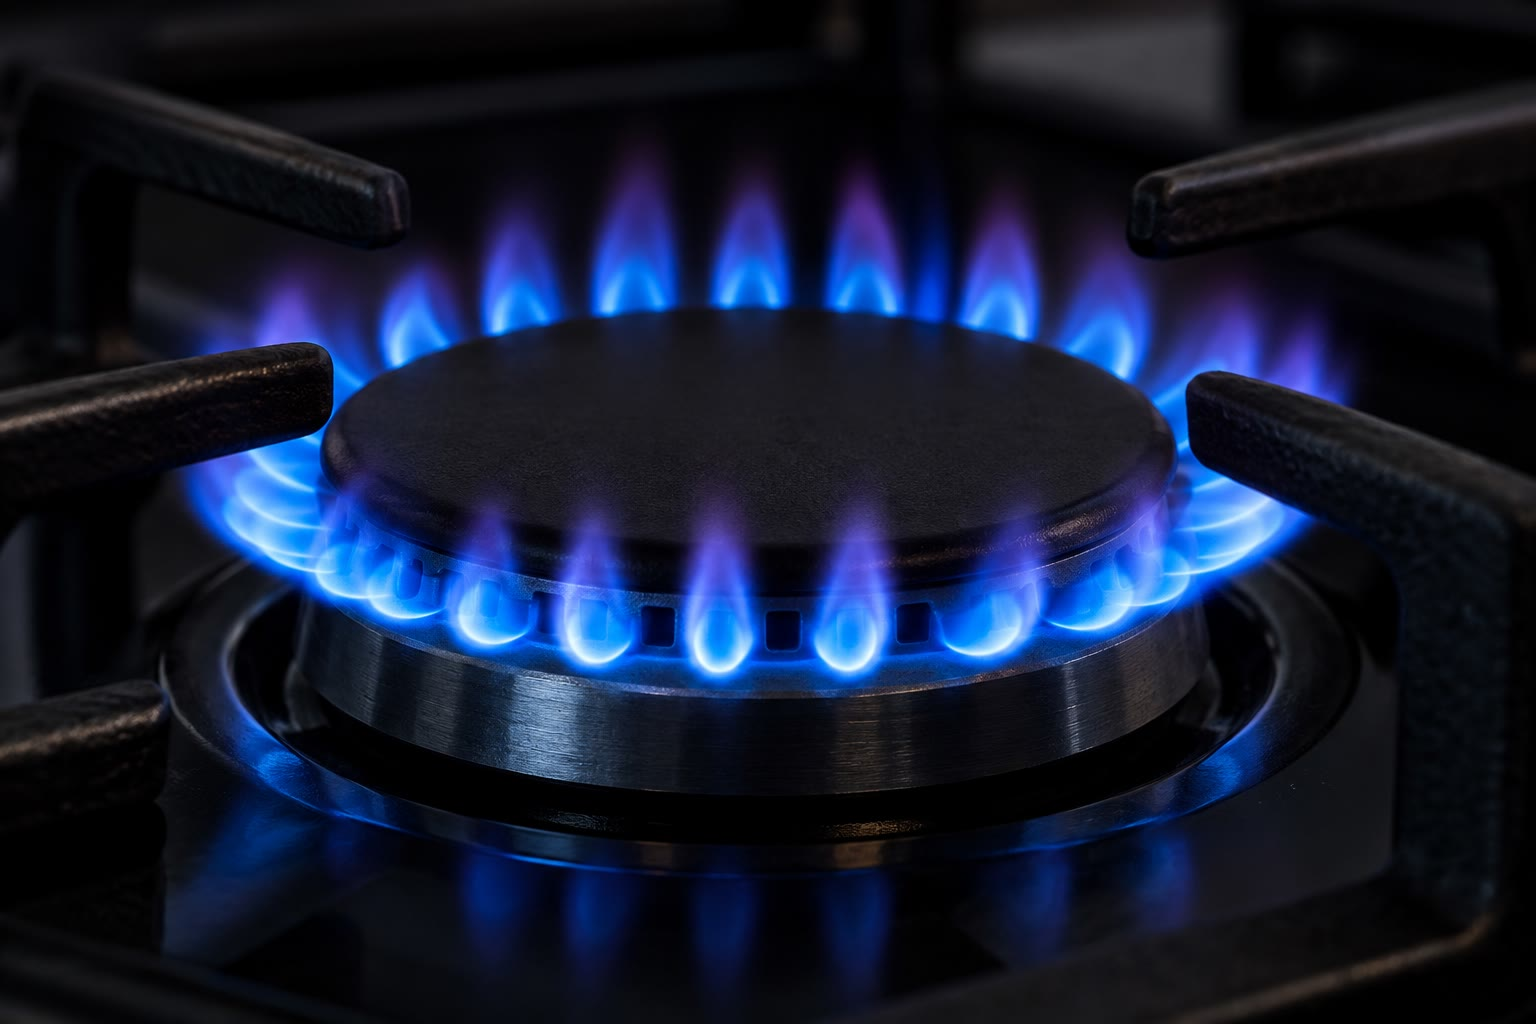
\includegraphics[width=0.5\linewidth]{images/book1/ai/g7-gas-flame.jpg}

{\small Nyala biru kompor gas: metana dalam gas alam sedang \omterm{def:g4:what-a-fire-needs:burning}{terbakar}.}
\end{omfigure}

\section{Model molekul}

\begin{remark}[Model, dan warna-warnanya]\label{rem:g7:atoms-and-molecules:models}
Para ahli kimia membuat \emph{model \omterm{def:g7:atoms-and-molecules:molecule}{molekul}} dengan bola untuk \omterm{def:g7:atoms-and-molecules:atom}{atom} dan
tongkat untuk ikatan di antaranya. Warna-warnanya adalah kesepakatan
yang dipakai di seluruh dunia --- karbon hitam, hidrogen putih, oksigen
merah, nitrogen biru --- dan bukan warna \omterm{def:g7:atoms-and-molecules:atom}{atom} yang sebenarnya: satu
\omterm{def:g7:atoms-and-molecules:atom}{atom} saja sama sekali tidak berwarna. Model juga memperlihatkan bentuk
\omterm{def:g7:atoms-and-molecules:molecule}{molekul}, yang tidak diperlihatkan oleh rumus: \omterm{def:g7:atoms-and-molecules:molecule}{molekul} air bengkok,
\omterm{def:g7:atoms-and-molecules:molecule}{molekul} karbon dioksida lurus.
\end{remark}

\begin{omfigure}
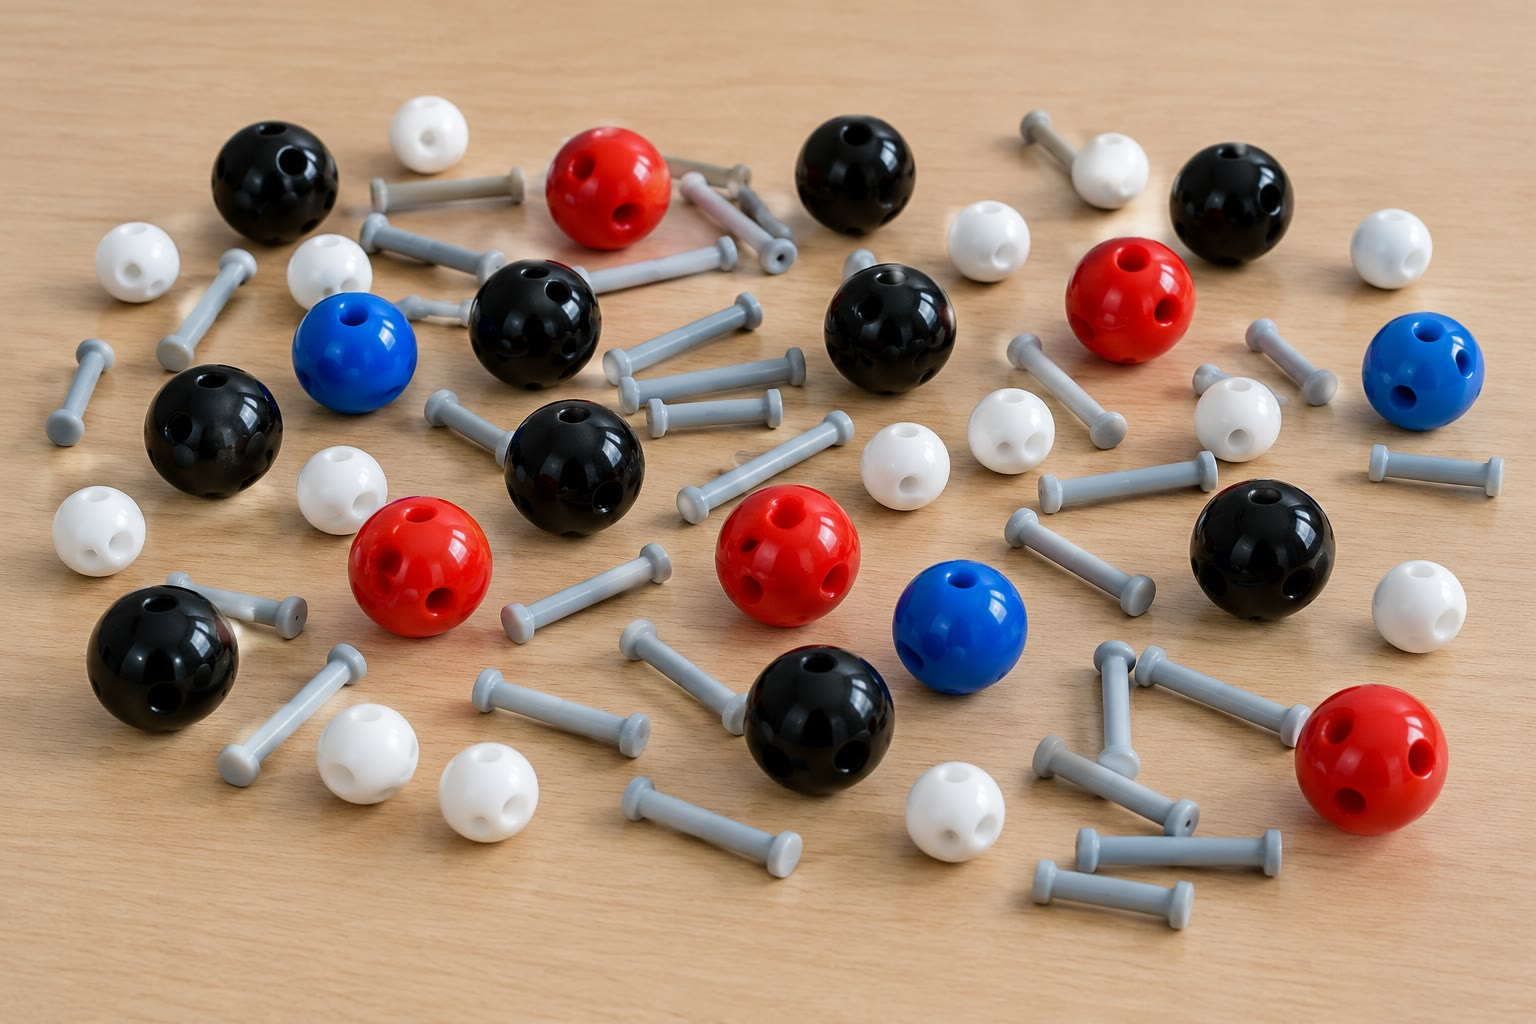
\includegraphics[width=0.5\linewidth]{images/book1/ai/g7-model-kit.jpg}

{\small Perangkat model \omterm{def:g7:atoms-and-molecules:molecule}{molekul}: bola untuk \omterm{def:g7:atoms-and-molecules:atom}{atom}, dengan lubang untuk
tongkat yang melambangkan ikatan.}
\end{omfigure}

\begin{method}[Dari model ke rumus]\label{met:g7:atoms-and-molecules:model}
Untuk menuliskan rumus sebuah \omterm{def:g7:atoms-and-molecules:molecule}{molekul} dari modelnya:
\begin{enumerate}
  \item kenali \omterm{def:g7:atoms-and-molecules:atom}{atom-atomnya} dari warnanya;
  \item hitung bola dari setiap warna;
  \item tuliskan \omterm{def:g7:atoms-and-molecules:symbol}{lambang-lambangnya} dengan jumlahnya sebagai \omterm{def:g7:atoms-and-molecules:formula}{angka
        indeks}, karbon lebih dulu, lalu hidrogen, lalu \omterm{def:g7:atoms-and-molecules:atom}{atom-atom} lain
        menurut urutan abjad \omterm{def:g7:atoms-and-molecules:symbol}{lambangnya}.
\end{enumerate}
Satu bola hitam yang tergabung dengan empat bola putih: satu karbon,
empat hidrogen, \ce{CH4}.
\end{method}

\section{Latihan}

\begin{exercise}[$\star$]\label{exo:g7:atoms-and-molecules:1}
Apa itu \omterm{def:g7:atoms-and-molecules:atom}{atom}? Apa itu \omterm{def:g7:atoms-and-molecules:molecule}{molekul}?
\end{exercise}

\begin{exercise}[$\star$]\label{exo:g7:atoms-and-molecules:2}
Tuliskan \omterm{def:g7:atoms-and-molecules:symbol}{lambang} hidrogen, karbon, nitrogen, oksigen, natrium, dan
besi.
\end{exercise}

\begin{exercise}[$\star$]\label{exo:g7:atoms-and-molecules:3}
Berapa \omterm{def:g7:atoms-and-molecules:atom}{atom} dari setiap jenis yang ada dalam satu \omterm{def:g7:atoms-and-molecules:molecule}{molekul} karbon
dioksida, \ce{CO2}? Berapa \omterm{def:g7:atoms-and-molecules:atom}{atom} seluruhnya?
\end{exercise}

\begin{exercise}[$\star$]\label{exo:g7:atoms-and-molecules:4}
Sebutkan nama \omterm{def:g7:atoms-and-molecules:molecule}{molekul} \ce{H2O}, \ce{O2}, \ce{CH4}, dan \ce{N2}.
\end{exercise}

\begin{exercise}[$\star$]\label{exo:g7:atoms-and-molecules:5}
Sebuah \omterm{def:g7:atoms-and-molecules:molecule}{molekul} nitrogen dioksida, gas cokelat yang terdapat di \omterm{def:g4:air-a-mixture-of-gases:air}{udara}
tercemar, tersusun atas satu \omterm{def:g7:atoms-and-molecules:atom}{atom} nitrogen dan dua \omterm{def:g7:atoms-and-molecules:atom}{atom} oksigen.
Tuliskan rumusnya.
\end{exercise}

\begin{exercise}[$\star\star$]\label{exo:g7:atoms-and-molecules:6}
Jelaskan perbedaan antara \ce{O2} dan \ce{2O}, serta antara \ce{CO}
dan \ce{Co}.
\end{exercise}

\begin{exercise}[$\star\star$]\label{exo:g7:atoms-and-molecules:7}
Berapa \omterm{def:g7:atoms-and-molecules:atom}{atom} hidrogen dan berapa \omterm{def:g7:atoms-and-molecules:atom}{atom} oksigen yang ada dalam
\ce{3H2O}? Dalam \ce{5O2}?
\end{exercise}

\begin{exercise}[$\star\star$]\label{exo:g7:atoms-and-molecules:8}
Sebuah model terdiri atas satu bola hitam yang tergabung dengan dua bola
merah. Sebutkan \omterm{def:g7:atoms-and-molecules:atom}{atom-atomnya}, tuliskan rumusnya, dan sebutkan nama
\omterm{def:g7:atoms-and-molecules:molecule}{molekulnya}.
\end{exercise}

\begin{exercise}[$\star\star$]\label{exo:g7:atoms-and-molecules:9}
Dalam tabel Dalton, air tersusun atas satu \omterm{def:g7:atoms-and-molecules:atom}{atom} hidrogen dan satu \omterm{def:g7:atoms-and-molecules:atom}{atom}
oksigen. Tuliskan rumus yang dimaksud Dalton, dan katakan berapa \omterm{def:g7:atoms-and-molecules:atom}{atom}
yang kurang pada \omterm{def:g7:atoms-and-molecules:molecule}{molekul} air menurut Dalton.
\end{exercise}

\begin{exercise}[$\star\star$]\label{exo:g7:atoms-and-molecules:10}
Apakah air murni sebuah \omterm{def:g6:pure-substances-and-mixtures:mixture}{campuran}? Apakah \omterm{def:g4:air-a-mixture-of-gases:air}{udara} \omterm{def:g6:pure-substances-and-mixtures:mixture}{campuran}? Jawablah dengan
menguraikan \omterm{def:g7:atoms-and-molecules:molecule}{molekul-molekul} yang dikandung masing-masing.
\end{exercise}

\begin{exercise}[$\star\star\star$]\label{exo:g7:atoms-and-molecules:11}
Sebuah \omterm{def:g7:atoms-and-molecules:atom}{atom} hidrogen berukuran sekitar sepersepuluh juta milimeter.
Berapa \omterm{def:g7:atoms-and-molecules:atom}{atom} hidrogen, dijajarkan berdampingan, yang membentuk garis
sepanjang \qty{1}{cm}? Dan garis sepanjang lapangan sepak bola,
\qty{100}{m}?
\end{exercise}

\begin{exercise}[$\star\star\star$]\label{exo:g7:atoms-and-molecules:12}
Glukosa, gula yang memberi makan sel-sel kita, memiliki rumus
\ce{C6H12O6}. Berapa \omterm{def:g7:atoms-and-molecules:atom}{atom} yang dikandung satu \omterm{def:g7:atoms-and-molecules:molecule}{molekul} glukosa? Berapa
persen di antaranya \omterm{def:g7:atoms-and-molecules:atom}{atom} hidrogen? Berapa persen \omterm{def:g7:atoms-and-molecules:atom}{atom} karbon?
\end{exercise}

\section{Soal: Atom-Atom dalam Satu Tarikan Napas}

\begin{problem}[{Soal akhir pekan --- menghitung atom dalam satu tarikan
napas udara, sebelum dan sesudah udara itu berada di paru-paru kita}]
\label{pb:g7:atoms-and-molecules:1}
% ledger: air:N2, air:O2, air:Ar (78.08 / 20.95 / 0.93 rounded to 78 / 21 / 1),
% breath:O2, breath:CO2, breath:N2 (expired air: 16 / 4 / 78, water vapour removed)
Nitrogen melewati paru-paru tanpa berubah, jadi nitrogen menjadi tolok
ukur yang baik. Dalam \omterm{def:g4:air-a-mixture-of-gases:air}{udara} kering, untuk setiap 78 \omterm{def:g7:atoms-and-molecules:molecule}{molekul} nitrogen
terdapat sekitar 21 \omterm{def:g7:atoms-and-molecules:molecule}{molekul} oksigen dan 1 \omterm{def:g7:atoms-and-molecules:atom}{atom} argon: seluruhnya 100
partikel (\omterm{def:g7:atoms-and-molecules:molecule}{molekul} atau \omterm{def:g7:atoms-and-molecules:atom}{atom} tunggal). Dalam \omterm{def:g4:air-a-mixture-of-gases:air}{udara} yang diembuskan,
setelah uap airnya dihilangkan, 78 \omterm{def:g7:atoms-and-molecules:molecule}{molekul} nitrogen yang sama disertai
sekitar 16 \omterm{def:g7:atoms-and-molecules:molecule}{molekul} oksigen, 4 \omterm{def:g7:atoms-and-molecules:molecule}{molekul} karbon dioksida, dan 1 \omterm{def:g7:atoms-and-molecules:atom}{atom} argon.

\medskip
\noindent\textbf{Bagian I --- \omterm{def:g4:air-a-mixture-of-gases:air}{Udara} yang kita hirup.}
\begin{enumerate}
  \item Tuliskan rumus \omterm{def:g7:atoms-and-molecules:molecule}{molekul} nitrogen, oksigen, dan karbon dioksida,
        dan berikan jumlah \omterm{def:g7:atoms-and-molecules:atom}{atom} dalam masing-masing.
  \item Argon dihitung dalam \omterm{def:g7:atoms-and-molecules:atom}{atom}, bukan dalam \omterm{def:g7:atoms-and-molecules:molecule}{molekul}. Apa yang
        ditunjukkan hal ini tentang argon?
  \item Dalam 100 partikel \omterm{def:g4:air-a-mixture-of-gases:air}{udara} yang dihirup ini, berapa \omterm{def:g7:atoms-and-molecules:atom}{atom} nitrogen
        yang ada? Berapa \omterm{def:g7:atoms-and-molecules:atom}{atom} oksigen?
  \item Berapa \omterm{def:g7:atoms-and-molecules:atom}{atom} seluruhnya dalam 100 partikel ini?
  \item Berapa persen \omterm{def:g7:atoms-and-molecules:atom}{atom-atom} ini yang berupa \omterm{def:g7:atoms-and-molecules:atom}{atom} nitrogen? Bulatkan
        ke bilangan bulat terdekat.
\end{enumerate}

\medskip
\noindent\textbf{Bagian II --- \omterm{def:g4:air-a-mixture-of-gases:air}{Udara} yang kita embuskan.}
\begin{enumerate}[resume]
  \item Dalam \omterm{def:g4:air-a-mixture-of-gases:air}{udara} embusan yang menyertai 78 \omterm{def:g7:atoms-and-molecules:molecule}{molekul} nitrogen yang
        sama, berapa \omterm{def:g7:atoms-and-molecules:atom}{atom} oksigen yang ada di dalam \omterm{def:g7:atoms-and-molecules:molecule}{molekul} oksigen? Di
        dalam \omterm{def:g7:atoms-and-molecules:molecule}{molekul} karbon dioksida? Seluruhnya?
  \item Bandingkan dengan soal 3. Berapa \omterm{def:g7:atoms-and-molecules:atom}{atom} oksigen yang hilang? Ke
        dalam \omterm{def:g7:atoms-and-molecules:molecule}{molekul} apa \omterm{def:g7:atoms-and-molecules:atom}{atom-atom} itu pergi, \omterm{def:g7:atoms-and-molecules:molecule}{molekul} yang dibuat tubuh
        dari hidrogen makanan dan di sini dibuang bersama uap air?
  \item Berapa \omterm{def:g7:atoms-and-molecules:atom}{atom} karbon yang ada dalam \omterm{def:g4:air-a-mixture-of-gases:air}{udara} yang dihirup? Dalam \omterm{def:g4:air-a-mixture-of-gases:air}{udara}
        yang diembuskan?
  \item \omterm{def:g4:air-a-mixture-of-gases:air}{Udara} tidak membawa \omterm{def:g7:atoms-and-molecules:atom}{atom} karbon ke dalam paru-paru. Dari mana
        \omterm{def:g7:atoms-and-molecules:atom}{atom-atom} karbon dalam embusan napas dapat berasal? (Pikirkan apa
        yang dipakai tubuh untuk hidup.)
  \item Berapa \omterm{def:g7:atoms-and-molecules:molecule}{molekul} oksigen yang hilang, dan berapa \omterm{def:g7:atoms-and-molecules:molecule}{molekul} karbon
        dioksida yang muncul?
\end{enumerate}

\medskip
\noindent\textbf{Bagian III --- Hitungannya.}
\begin{enumerate}[resume]
  \item Uraikan model bola dan tongkat dari masing-masing keempat jenis
        partikel dalam \omterm{def:g4:air-a-mixture-of-gases:air}{udara} embusan, beserta warna bola-bolanya (argon
        digambarkan sebagai satu bola biru pucat).
  \item Berapa \omterm{def:g7:atoms-and-molecules:atom}{atom} seluruhnya dalam \omterm{def:g4:air-a-mixture-of-gases:air}{udara} embusan yang sudah
        dikeringkan? Berapa \omterm{def:g7:atoms-and-molecules:atom}{atom} lebih banyak daripada \omterm{def:g4:air-a-mixture-of-gases:air}{udara} yang
        dihirup? Jelaskan selisih itu dengan \omterm{def:g7:atoms-and-molecules:atom}{atom} karbon yang bertambah
        dan \omterm{def:g7:atoms-and-molecules:atom}{atom} oksigen yang hilang.
\end{enumerate}
\end{problem}
